\documentclass{article} % For LaTeX2e

\usepackage{nips14submit_e,times}
\usepackage{hyperref}
\usepackage{url}
\usepackage{graphicx}

\usepackage{listings}
\usepackage{color}

\definecolor{lightgray}{rgb}{1,1,1}
\definecolor{darkgray}{rgb}{.4,.4,.4}
\definecolor{redstrings}{rgb}{0.64,0.08,0.08}
\definecolor{blue}{rgb}{0,0,1}
\definecolor{greencomments}{rgb}{0,0.5,0}
\definecolor{cyan}{rgb}{0.0,0.6,0.6}

\renewcommand{\lstlistingname}{Code fragment}


\lstdefinelanguage{JavaScript}{
  keywords={break, case, catch, continue, debugger, default, delete, do, else, finally, for, function, if, in, instanceof, new, return, switch, this, throw, try, typeof, var, void, while, with, null},
  keywordstyle=\color{blue}\bfseries,
  ndkeywords={class, export, boolean, throw, implements, import, this},
  ndkeywordstyle=\color{blue}\bfseries,
  identifierstyle=\color{black},
  sensitive=false,
  comment=[l]{//},
  morecomment=[s]{/*}{*/},
  commentstyle=\color{greencomments}\ttfamily,
  stringstyle=\color{redstrings}\ttfamily,
  morestring=[b]',
  morestring=[b]"
}

\lstset{
   language=JavaScript,
   backgroundcolor=\color{lightgray},
   extendedchars=true,
   basicstyle=\footnotesize\ttfamily,
   showstringspaces=false,
   showspaces=false,
   numbers=left,
   numberstyle=\footnotesize,
   numbersep=9pt,
   tabsize=2,
   breaklines=true,
   showtabs=false,
   captionpos=b
}


%\documentstyle[nips14submit_09,times,art10]{article} % For LaTeX 2.09


\title{Inspecting community evolution using text and network structure}


\author{
Mario Karlovcec, Jan Rupnik, Primoz Skraba \\
Department of Computer Science\\
Jožef Stefan Institute\\
Jamova cesta 39, Ljubljana, Slovenia \\
}

% The \author macro works with any number of authors. There are two commands
% used to separate the names and addresses of multiple authors: \And and \AND.
%
% Using \And between authors leaves it to \LaTeX{} to determine where to break
% the lines. Using \AND forces a linebreak at that point. So, if \LaTeX{}
% puts 3 of 4 authors names on the first line, and the last on the second
% line, try using \AND instead of \And before the third author name.

\newcommand{\fix}{\marginpar{FIX}}
\newcommand{\new}{\marginpar{NEW}}

% \nipsfinalcopy % Uncomment for camera-ready version

\begin{document}


\maketitle

\begin{abstract}
Detect communities in several timestamps, connect them in neighbouring timestamps, extract keywords in communities and analyse structure and topic change.
\end{abstract}

\section{Introduction}

In this work we propose an approach for detecting, visualizing and modelling community evolution of dynamic networks using textual features and graph structure. The approach is implemented in QMiner – open source data analytics platform for processing streams of structured and unstructured data \footnote{http://qminer.ijs.si/}. QMiner integrates machine learning algorithms with network analysis based on SNAP library \cite{snap}.

Mapping between communities and clusters.

Building community evolution model.

Predict splits and merges.

Examine homophony and heterogeneity.

Use hub nodes (page rank, centrality, etc.) members to track communities/clusters.

K-means clustering (e.g. num. of communities in t for K)

Keywords extraction for community description

Communities are often defined using the network topology as groups of nodes with many links inside the groups but a few links between them . Finding communities is looking for a partition of the nodes that maximizes a quality function which captures the idea of dense groups communities \cite{aynaud}. One such broadly used quality function is modularity \cite{newman2003}.

\section{Related work}

Communities in evolving networks are usually analysed using the following three groups of methods: (1) using static algorithms on several snapshots and connecting the resulting communities, (2) using temporal information directly in community detection methods and (3) using incremental/online algorithms \cite{aynaud}. In this work we apply the first approach of independently computing communities, following by solving community matching/tracking problem to obtain the community evolution. Positive side of this approach is that the static version of this problem is well studied and there are many algorithm developed (Clauset-Newman-Moore\cite{clauset-newman-moore}, ...). The downside of the approach is related to instability \cite{aynaud2010}. Since the algorithms are often non deterministic, small modification of the input network may lead to many changes in the resulting community partition.
 
Identifying relationship between the neighbouring partitions is called matching or tracking problem and it is a crucial step in using static algorithms on dynamic networks.
MONIC \cite{spiliopoulou} is a generalized methodology for modelling and tracking external and internal cluster transitions, that include: survival, split into multiple clusters, absorption, disappearing and emergence of a new cluster. In line with the set theory approach of  MONIC methodology, in \cite{gliwa2013} authors determine matching of cluster by calculating modified Jaccard coefficient, with an additional constraint on difference in cluster sizes. Other approaches of solving the matching problem include using key nodes in the clusters \cite{wang} and community detection algorithms for the matching problem\cite{palla}.

Topic evolution graph to trace topic transitions \cite{mei2005}.
Predicting community evolution problem is tackled in \cite{gliwa2013}. Predictions are based on the previous events in group lifetime described by group size, cohesion, leadership and density.

\section{Approach}
Communities of each snapshot of a dynamic graph are detected using any of the statical community detection algorithm. Communities are then matched and a directed graph representing community evolution is constructed. Keywords are extracted from the text assigned to the nodes in the input graph snapshots to describe the content of the communities. Community evolution is visualized as a directed graph, using different colours and sizes of nodes and arcs. Based on the textual descriptions of clusters and the graph structure feature set for building classification model is constructed.

\begin{figure}\label{architecture}
   	\begin{center}
   	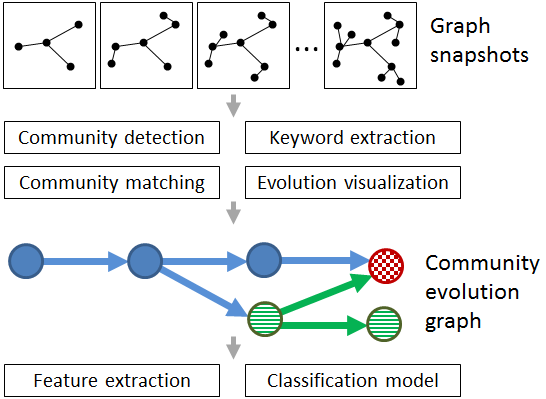
\includegraphics[width=0.6\textwidth]{architecture.png}
   	\end{center}
   	\caption{Approach}
\end{figure}
\subsection{Community detection and matching}
Input for the proposed approach is a set of snapshots of a evolving graph. A statical community detection algorithm is applied on each snapshot. Type of supported input snapshot graphs depends on the community detection algorithm. These are usually undirected or directed, weighed or unweighed graphs. The approach is independent of the choice of the community detection algorithm, making it modular and applicable on the wide range of different algorithms. Communities as groups of members obtained from each snapshot is an input for the community matching. Community matching problem can be reduced to determining whether a community in time t exists in time t+1 and to which community it maps to if it exists. This is determined by calculating Modified Jaccard measure (similar as in \cite{gliwa2013})  between each pair of neighbouring communities. If $A$ is a community at $t$ of size $|A|$ and $B$ is a community at $t+1$ of size $B$, then:
\begin{equation}
\alpha = \frac{A\cap B}{|A|},
\beta = \frac{A\cap B}{|B|}.
\end{equation}
If there is a pair of communities $A$ and $B$ such that $alpha$ and $beta$ are greater than two thresholds restricted to the interval $[0.5, 1]$, community $B$ represents the continuation of $A$ at $t+1$. Otherwise, if there is no match, community $A$ decays at $t$ and $B$ is a new community emerged at $t+1$. 

\subsection{Keyword extraction}
Keyword extraction process is conducted by uniting textual descriptions of nodes of a community into documents. Since the members of the communities change over time, a separate document is generated for each occurrence of a community. Next step is creating bag-of-words feature space representation of the collection of documents, where each document is a vector of n-grams. Bag-of-words representations of documents are created by tokenization, stop-words removal, stemming using English Porter stemmer, tf-idf weighting and normalization. Final step of the keyword extraction process is to select an arbitrary number (in our experiments usually 10) of n-grams with highest tf-idf scores from each documents. These n-grams are the keywords that represent the content of communities.

\subsection{Visualization}
An important part of this work is visualization of the community evolution. This enables inspecting interesting events in graph evolution, like sudden splits and merges of communities. Imagine a stable community evolution with few communities and rear splits and merges, which at a point in time explodes with many splits and emergence of new communities. Such case indicates an atypical change in structure that could be easily identified with a visualization. Evolution of communities is visualized as a directed graph, with nodes representing communities and arcs showing the relationships between communities in consecutive time points. Arcs are drawn whenever two neighbouring communities share common members. Size of the nodes corresponds to the number of member of communities, while width of the arcs fits the number of shared members and is relative to the diameter of the nodes. Colour is used to indicate whether two connected neighbouring nodes represent the same community. Keyword obtained in the keywords extraction step and assigned to the nodes in the directed graph, improve the interpretation of evolution by giving information on content of communities.
 
\subsection{Feature extraction}
For building community evolution model we use both features extracted from text assigned to communities, as well as features from the graph structure. Text based features are constructed by performing text based clustering of community members at time $t$ and mapping between communities and clusters. At each time point all the members that are in any of the community are represented using the bag-of-words feature vector representation. This process is similar as in keywords extraction step, but instead of grouping the members of the same communities, here each member is represented as a separate BOW vector. One of the clustering method is used to cluster the member based on text. If the method requires a parameter for specifying the number of clusters (e.g. K-means), the number of communities at time point $t$ is used. After clustering, mapping between each community and cluster is performed. Each community gets a vector with number of elements corresponding to the number of clusters it maps to. The values of the vector are proportions of elements from a community mapped to a cluster. This vector is the basis for deriving two features: (1) {\bf number of significant clusters it maps to} and (2) { \bf uniformity of the mapping}.

The first feature counts the number of mappings greater than a threshold restricted to the interval $[0, 1]$. In the experiments we used $K^{-1}$, where K is  the number of communities at time point $t$. The second feature, uniformity of the mapping distribution is calculated using Shannon's entropy formula.

Graph structure based features are: centralization \cite{freeman1978}, density\cite{wasserman1994}, cohesion and group size.

\section{Experimental results}
Build community evolution model.
Use the model for prediction on different datasets (co-authoring, companies, ...). Evaluation

\begin{table}[t]
\caption{Sample table title}
\label{sample-table}
\begin{center}
\begin{tabular}{ll}
\multicolumn{1}{c}{\bf Dataset}  &\multicolumn{1}{c}{\bf DESCRIPTION}
\\ \hline \\
Dendrite         &Input terminal \\
Axon             &Output terminal \\
Soma             &Cell body (contains cell nucleus) \\
\end{tabular}
\end{center}
\end{table}

\section{Conclusion and discussion}

\subsubsection*{Acknowledgments}
   The authors gratefully acknowledge that the funding for this work was provided by the project X-LIKE (ICT-257790-STREP)\cite{xlike}.


\bibliographystyle{unsrt}
\bibliography{communities}

\end{document}